\chapter{Design\label{cha:chapter4}}
Against the background of the requirements described previously in chapter 3, this chapter provides a design concept for the framework. Section 4.1 will describe a basic architectural concept of the framework to be refined in section 4.2 and 4.3 which provide a more detailed description of the framework's components and their interactions. The final section reviews the parity between the requirements from chapter 3 and the corresponding architectural components. 
        


\section{Architecture Overview\label{sec:des_ar_ov}}
Figure \ref{fig:arch_overview} shows an architecture overview of the framework, which consists mainly of seven components. The components with three dots(...) in them means that the framework can be later extended with new components for adding new services to the framework like SUBSCRIBE/NOTIFICATION.

\begin{figure}[htb]
  \centering
  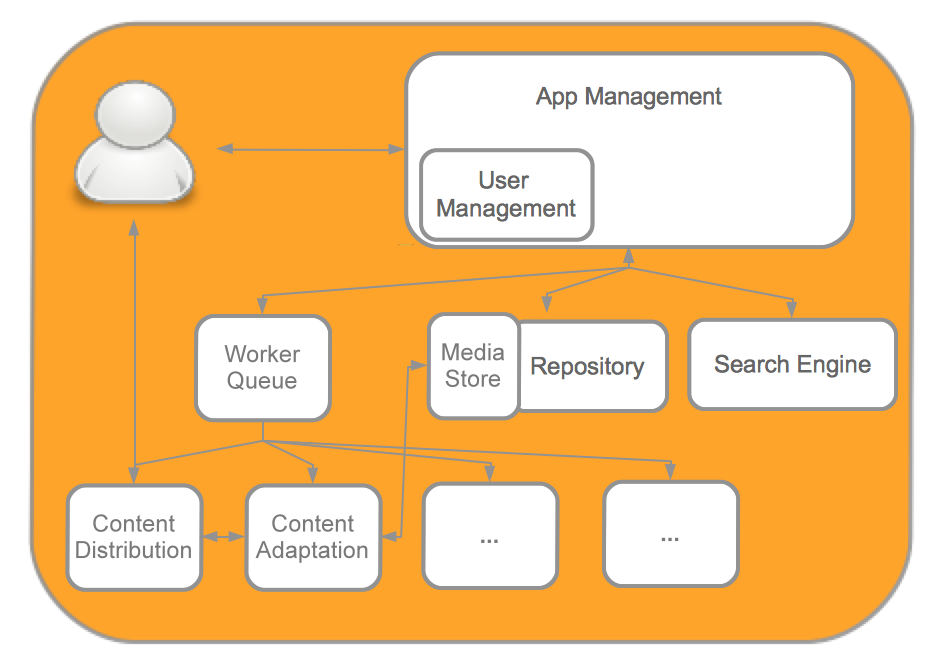
\includegraphics[scale=0.6]{arch_overview.png}\\
  \caption{Architecture Overview}
  \label{fig:arch_overview}
\end{figure}

The App Management component is the main entry for each developer to interact with the framework. These developers needs to authenticate them self in order to use the framework and therefore a User Management component is needed. Furthermore the Repository/Media Store is also needed for     
\section{Framework Components\label{sec:des_com}}
\subsection{App Management\label{sec:des_repo}}
\subsection{User Management}
\subsection{Repository\label{sec:des_repo}}
\subsection{Search Engine\label{sec:des_se_en}}
\subsection{Content Adaptation\label{sec:des_ar_ov}}
\subsection{Content Distribution\label{sec:des_cdn}}	
	
	\subsection{Application Messaging\label{sec:des_me}}
	
	\subsection{User API\label{sec:des_api}}

\section{Interfaces\label{sec:des_inter}}

\section{Requirement Fulfillment\label{sec:des_inter}}